What do we need to create a 2 dimensional jump and run game? First of all we need a physics engine to recreate a realistic environment. Then we need a game engine to build our game on. After that we need the game itself and an environment creator to randomly generate the worlds.\bigskip\\
Now we need an AI. But how do we connect the AI with the game? How can the AI controll the player? How can the AI see where the next block is? That's where the Application Programming Interface (API) steps in. With this connection the AI can easily read the environment and move the player. Lastly we ``just'' need the AI algorithms.

\begin{figure}[H]
  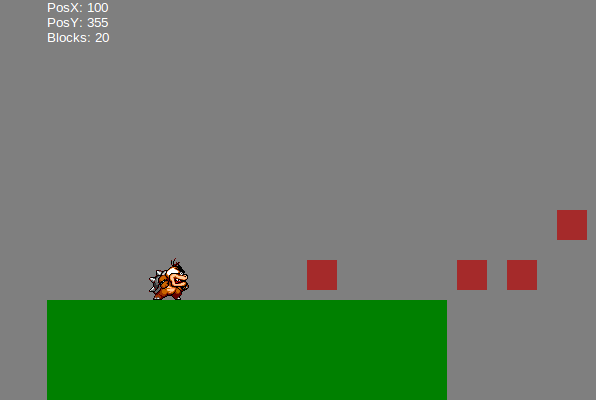
\includegraphics[width=0.45\textwidth]{images/game.png}
  \caption{The final game at the start point.}
\end{figure}
\newpage

\section{Physics Engine}
A physics engine is able to recreate an entire physical system like our world. They are mostly common in animated films, scientific experiments and video games. The gravity is the biggest part to cover. There are less and more accurate engines. In some the falling objects get faster or the objects can break when they fall on a solid ground.

\subsection{Gravity Example}
A block gets thrown horizontally with the force F. This block has now the force from the throw (horizontally) and from the gravity (vertically).\bigskip\\

\begin{figure}[H]
  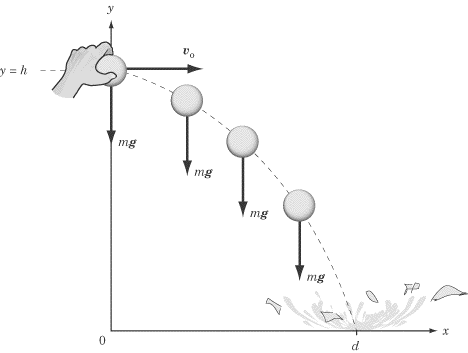
\includegraphics[width=0.45\textwidth]{images/gravity_example.png}
  \caption[Gravity example from \url{http://www.sparknotes.com/testprep/books/sat2/physics/chapter7section1.rhtml}]{Example for gravity.}
\end{figure}

\subsection{Collision Example}
A block gets thrown horizontally with the force F and collides with another, steady one with the same size and weight. After the collision the first block will fly back with half the force, while the other one gets pushed away with the other half of the force.

\begin{figure}[H]
  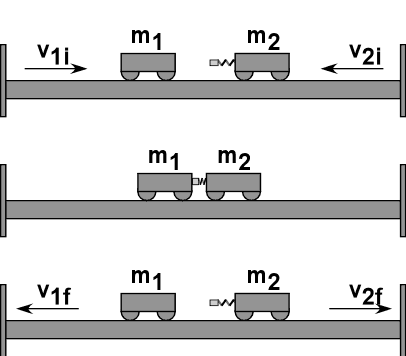
\includegraphics[width=0.45\textwidth]{images/collision_example.png}
  \caption[Collision example from \url{http://physicslearning2.colorado.edu/pira/resources/physics-testlecture-drawings}]{Example for a collision.}
\end{figure}

\subsection{Types of Physics Engines}
There are two main types of physics engines. The high-precision and the real-time engines:
\begin{description}
  \item[high-precision] This type of engine is used for exact copies of a physical system. They are mostly common for animations that must be very precise like scientific studies or animated films. It does not matter in this animations how many resources where used while rendering because you can let the machine run for many hours rendering the world and than analyze the result at the end.\smallskip\\
    To wrap it up: Those engines need much processing powers but are very precise. \ul{Quality before quantity}.
  \item[real-time] This type of engine is used for interactive animations like video games. The artificial physics must be calculated immediately. Unlike the high-precision engines this type of engine does not need much processing power, for it is minimized.\smallskip\\
    To wrap it up: The real-time engines do not need much processing power but are not very accurate. \ul{Quantity before quality}.
\end{description}

\subsection{What do we need?}
\begin{description}
  \item[collision] We need to be able to check for a collision between the player and a block above the ground.
  \item[gravity] We need to be able to use gravity for the player to jump and fall down. 
  \item[real-time] We are creating a game, so we need in the first place a fast engine.
\end{description}
\subsection{Setting Boundaries}
But let us stop here. Even though it is a really interesting topic, it is too extensive to go into the details. If you would like to know more, there are plenty of comprehensive studies about physics engines.
\newpage

\section{Game Engine}
We want the physics engine to create a game. But how can one do this? All by himself? No, we need to find a link between the game and the physics engine. This is where the game engine has a turn. It offers the opportunity never to touch the physics engine and to make the step from a world with just moving objects to a world, controlled by a human.
\subsection{What does a Game Engine?}
\begin{itemize}
  \item It unburdens the interaction between the human's controls like a keystroke or a mouse click and the animations that can be seen on the display.
  \item It eases the animations of the objects. For example when the player walks then should the character animate this movement.
  \item It implements the element of sound. With this feature you can easily add background music and/or sound effects.
  \item They are mostly specialized on 2D or 3D worlds. 3D worlds are way more complicated but they are more realistic.
  \item They are either built for a specific platform or they can compile the same source code for multiple platforms. For example if it supports multiple platforms you can create a game and run it on Windows, Linux, Xbox and PlayStation.
  \item Some engines even include a AI system to help building one. They often helps with the data logistics and sensor access.
\end{itemize}

\subsection{Examples of Game Engines}
\begin{description}
  \item[CryENGINE] A engine created by Crytek. It runs on PS3, Xbox 360 and PC. It has an advanced AI system with sensors like sight and hearing. The games Crysis, FarCry and Warface are the most famous of many.
  \item[Unreal Engine] A engine created by Epic Games. It runs on PC, PS3, Xbox 360, Wii U, PSVITA, Android, iOS and Flash. The Unreal AI is also advanced and includes a special navigation mesh system to optimize the performance and memory usage. Dishonored, Gears of War, Batman: Arkham City and Mass Effect are the best examples for this engine.
  \item[Anvil] Until 2006 it was known as Scimitar and is created by Ubisoft. It runs on PC, PS3, Xbox 360, Wii U and PSVITA. Prince of Persia, Assassin's Creed and Tom Clancy's Rainbow 6: Patriots are the most known examples for this engine.
  \item[IW Engine] A engine created by Infinity Ward. It runs on PC, PS3, Xbox 360, Wii and Wii U. The complete Call of Duty series expect the first one is based on this engine.
  \item[Blender] This is the most popular open source game engine. 
\end{description}

\subsection{What do we need?}
We don't need a complex game engine for we are creating a simple, 2 dimensional game. It should just cover the basic necessities like:
\begin{itemize}
  \item interaction between user interface and animations
  \item animations for the objects
  \item sound implementations
  \item built for PC only should be sufficient
  \item 2 dimensional
\end{itemize}
\newpage

\section{The Game}
For it would take too much time to create an own physics and game engine, we decided to use the open source engine Crafty. It is based on the programming language JavaScript allowing the game to run in a modern web browser.

\subsection{Goal}
  We want to create a game with this specifications:
  \begin{itemize}
    \item 2 dimensional
    \item jump and run
    \item blocks to jump on
    \item gaps in the floor to fall down
    \item randomly generated
    \item generator ensures that the game is solvable
    \item finish line at the end of the parcour
    \item die from falling down
    \item win from reaching the finish line
    \item after winning or dying: restart the game
  \end{itemize}

\subsection{Basic Composition}
We used an event-driven development architecture. That means that the engine triggers events and we define what should happen.\bigskip\\
Here is the main structure of the game in a theoretically programming language:
\begin{verbatimtab}
When the player hits a solid object:
  The player stops moving

When the player hits a deadly area:
  The player dies
  Restart the game

When the player hits the finish line:
  The player wins
  Restart the game
\end{verbatimtab}


\subsection{Animation Sprites}
To bring life to our player we decided to use a sprite. A sprite is basically a collection of images with the same character but in different positions. You just have to decide which of them belongs to which movement.\bigskip\\

\begin{figure}[H]
  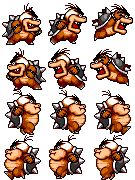
\includegraphics{images/player.png}
  \caption{The sprite to animate our player.}
\end{figure}

\begin{description}
  \item[standing right] If the player stands and looks to the right the game should use the image from \ul{row 1 the first}
  \item[standing left] If the player stands and looks to the left the game should use the image from \ul{row 2 the first}
  \item[jumping right] If the player jumps to the right the game should use the image from \ul{row 1 the last}
  \item[jumping left] If the player jumps to the left the game should use the image from \ul{row 2 the last}
  \item[walking right] If the player walks to the right the game should switch through all images from \ul{the third row}
  \item[walking left] If the player walks to the left the game should switch through all images from \ul{the forth row}
\end{description}

\newpage
\subsection{Environment Creator}
Our environment consists of blocks and a floor with gaps. We now need a creator that generates random environments. To make it consistent we chose that all blocks have the same size. They are in one of this three heights:
\begin{enumerate}
  \item The height of the player. Easy to jump on.
  \item Twice the height of the player. The maximal height to jump on.
  \item Thrice the height of the player. Just reachable from a block from the first or second height.
\end{enumerate}
\begin{figure}[H]
  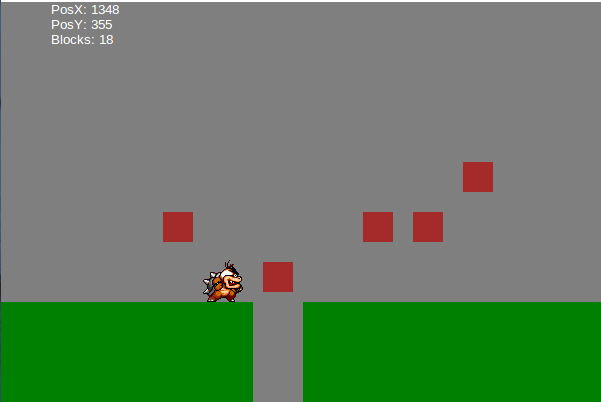
\includegraphics[width=0.45\textwidth]{images/block_heights.png}
  \caption{The three possible block heights.}
\end{figure}
The gaps in the floor exist in three different sizes:
\begin{description}
  \item[one block] These gaps are very easy to jump over.
  \item[two blocks] These are a little harder, but should pose no problem.
  \item[three blocks] These are the most difficult ones. To jump over them you have to stand on the very last corner of the floor or on a block.
\end{description}
\begin{figure}[H]
  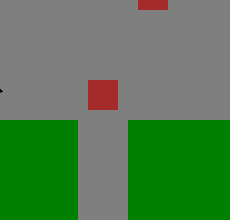
\includegraphics[width=0.145\textwidth]{images/gap_size1.png}
  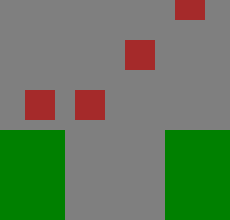
\includegraphics[width=0.145\textwidth]{images/gap_size2.png}
  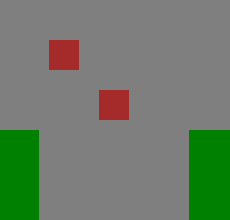
\includegraphics[width=0.145\textwidth]{images/gap_size3.png}
  \caption{The three possible sizes of the gaps.}
\end{figure}

\subsubsection{Prevent Unsolvable Environments}
Basically we could just say ``create some blocks and some gaps in the ground'' but it would most likely get unsolvable. To prevent this we have chosen this insurances to prevent that:
\begin{itemize}
  \item The blocks from the first or second height are no problem for the player to jump on.
  \item The blocks on the third height may not exist if they don't have an accessible block from the first or second height. This is to make sure that the player can jump on every block.
  \item The gaps may not be bigger than the player could jump. 
\end{itemize}

\subsubsection{Composition}
This is the basic composition of the creator in a theoretical programming language:
\begin{verbatimtab}
Define the start point
Until the whole width of the field is used:
  Set a random end point
  Create a ground from the start to end point
  Get a random gap width (1, 2 or 3)
  Set the start point: end point + gap width

15 times:
  Until the x-coordinate is unique:
    Generate random x-coordinate

  Get a random height of 1 or 2
  Generate the block from x and the height

  With a probability of 3:
    Generate a next block with the height 3
\end{verbatimtab}


\newpage
\section{Application Programming Interface (API)}
As mentioned before we need to create an interface for the AI to control the player and read the environment. To gain full control we need actors and sensors.\medskip\\
For the human the actors are the keys and his fingers with which he can handle the player. The sensors are the monitor and his eyes. With this he can analyze what is happening.\medskip\\
Now we have to adapt those actors and sensors to our API.
\subsection{Actors}
The actors are responsible for the actions of the player. We need those available actions:
\begin{description}
  \item[jump] The AI must be able to jump to the left and the right.
  \item[walk] The AI must be able to walk to the left and the right.
\end{description}

\subsection{Sensors}
The sensors are responsible for the measuring of the environment. We need those available sensors:
\begin{description}
  \item[won?] Did the player win?
  \item[died?] Did the player die?
  \item[my position] Where is the position of the player?
  \item[nearest block] Where is the nearest block?
  \item[all blocks] Where are all blocks? This is needed to plan a few steps further
  \item[nearest gap] Where is the nearest gap?
  \item[all gaps] Where are all gaps?
  \item[finish line] Where is the finish line? To check if the AI is going in to the right direction.
\end{description}
\subsection{Implementation}
Those actors and sensors sound all very logical but how could we implement those?\medskip\\
For the sensors we just have to access the created elements. Of course they need to be well formed and easily accessible. For the nearest gap or block we just have to iterate through all and check which of those the closest one is.\medskip\\
For the actors it is more complicated. We have to include multiple callbacks and helper variables to ease the access. For example we need a callback that will be triggered when the player lands on the ground or when he have reached the desired distance.
\newpage
\section{Our Artificial Intelligence (AI)}
